\documentclass{slides-template}

%%% Packages
\usepackage[textsize=small]{todonotes}
\usepackage{subcaption}
\usetikzlibrary{3d, arrows.meta, positioning}
\usepackage{tabularray}
\UseTblrLibrary{amsmath,booktabs,counter,diagbox,nameref,siunitx,varwidth,zref}
\pgfkeys{tikz/.cd,
box color/.code={\xdef\tkzThreedBoxColor{#1}},
box color=white
}
\def\parsexy(#1,#2,#3){(#1,#2)}
\def\parsexz(#1,#2,#3){(#1,#3)}
\def\parseyz(#1,#2,#3){(#2,#3)}
\def\parsex(#1,#2,#3){#1}
\def\parsey(#1,#2,#3){#2}
\def\parsez(#1,#2,#3){#3}

\newcommand{\tkzThreeDBox}[5][white]{\tikzset{#1}
\edef\temp{%
\noexpand\filldraw[#1,fill=\tkzThreedBoxColor!40,canvas is yz plane at x=\parsex#3+\parsex#2] 
\parseyz#2 rectangle (\parsey#4+\parsey#2,\parsez#5+\parsez#2);
\noexpand\filldraw[#1,fill=\tkzThreedBoxColor!30,canvas is xz plane at y=\parsey#4+\parsey#2] 
\parsexz#2 rectangle (\parsex#3+\parsex#2,\parsez#5+\parsez#2);
\noexpand\filldraw[#1,fill=\tkzThreedBoxColor!50,canvas is xy plane at z=\parsez#5+\parsez#2] 
\parsexy#2 rectangle (\parsex#3+\parsex#2,\parsey#4+\parsey#2);
}
\temp
}


\usepackage{caption}
\setlength{\textfloatsep}{10pt plus 1.0pt minus 2.0pt}
\setlength{\floatsep}{6pt plus 1.0pt minus 2.0pt}
\captionsetup{aboveskip=6pt}

\def\div{\mathrm{div}}
\def\O{\mathcal{O}}
\newcommand{\norm}[1]{\left\lVert#1\right\rVert}

\bibliography{slides.bib}
\title[Geodesic Paths and Distances on Meshes]{Geodesic Paths and Distances on Meshes\texorpdfstring{:\\ PDE 
    and Computational Geometry Approaches}{}}

\author{Matthieu Pierre Boyer \& Antoine Groudiev}

%%% Preamble
\def\abs#1{\left|#1\right|}
\def\R{\mathbb{R}}

\def\V{\mathbb{V}}
\def\nv{n_{\V}}
\def\E{E}
\def\ne{n_{\E}}
\def\F{\mathcal{F}}
\def\nf{n_{\F}}
\def\d{\mathrm{d}}

\def\imp#1{\textcolor{purple}{\bfseries #1}}

\newcommand\intertitre[1]{%
	\SetRow{rowsep=1pt,bg=teal!10}
	\SetCell[c=5]{mode=text,l,font=\itshape\footnotesize}
	#1 &
}

\begin{document}
\maketitle

\begin{frame}{Introduction}
	\centering
	\includegraphics[height=3.4cm]{../report/images/rabbit-paths.png}
	\hspace{.5cm}
	\includegraphics[height=3.4cm]{../report/images/venus-paths.png}
	\hspace{.5cm}
	\includegraphics[height=3.4cm]{../report/images/star-paths.png}
\end{frame}
%
%
\begin{frame}{Problem Positioning}
	\begin{center}
		Given a mesh of a $2$-manifold embedded in $\mathbb{R}^{3}$ and two points on the mesh, what is the shortest path between the points?
	\end{center}
	\pause
	\textbf{$2$-Manifold:} a surface that looks locally like $\R^{2}$;\\\pause
	\textbf{Mesh:} a set $\V$ of vertices, a set $\F$ of faces in $\V^{3}$.
	\begin{figure}
		\centering
		\includegraphics[width=.28\linewidth]{../report/images/manifold.png}
		\includegraphics[width=.3\linewidth]{../report/images/nonmanifold.png}
		\caption{Examples of a $2$-manifold (left) and non-manifold (right) mesh.}
	\end{figure}
\end{frame}

\section{PDE Methods}
\begin{frame}{Discrete Differential Geometry}
	The Laplace-Beltrami operator of a function $u$ is given by:
	\begin{equation}
		(\Delta u)_{i} = \frac{1}{2A_{i}}\sum_{e = (i, j)}\left(\cot \alpha_{i, j} + \cot \beta_{i, j}\right)\left(u_{i} - u_{j}\right).
	\end{equation}
	It quantifies the symmetric deviation of the variation of the value at a point.
\end{frame}

\begin{frame}{Physical Equations}
	We base ourselves on equations modelling the propagation of a phenomenon:
	\begin{description}
		\item[Heat Equation] $\delta u_{t} = \frac{\d}{\d t}u_{0}$;
		\item[Poisson Equation] $\Delta u = u_{0}$ for a fixed distribution $u_{0}$;
		\item[Spectral Embedding] $\ell^{2}$ distance based on eigenspaces of the laplacian $\Delta$.
	\end{description}
\end{frame}

\begin{frame}{Fast Marching}
	We compute a variation of Dijkstra's algorithm based on the Eikonal equation $\abs{\nabla u} = 1$ for
	wavefront propagation.
	\begin{center}
		\usetikzlibrary{shadings}

\begin{tikzpicture}[x={(1, -.2)},z={(.4, .5)},y={(0, 1)}]
	\coordinate (origin) at (0, 0, 0);
	\draw[canvas is xy plane at z=0, ->] (origin) -- +(0, 2) node[above] {$\phi(x)$};
	\draw[canvas is xz plane at y=0] (origin) rectangle +(4, 4);
	%
	\coordinate[canvas is xz plane at y=0] (xi) at (.5, 0, 2.1);
	\coordinate[canvas is xz plane at y=0] (xj) at (3, 0, .6);
	\coordinate[canvas is xz plane at y=0] (xk) at (3.5, 0, 3.1);
	% Draw the triangle
	\fill[canvas is xz plane at y=0, thick, teal!50!purple!20!white] (xi) -- (xj) -- (xk) -- cycle;

	% Draw circles at vertices
	\fill (xi) circle (0.10) node[below left] {$x_i$};
	\fill (xj) circle (0.10) node[below right] {$x_j$};
	\fill (xk) circle (0.10) node[right] {$x_k$};
	%
	\coordinate[canvas is xz plane at y=0] (fxi) at ($(xi) + (0, .9, 0)$);
	\coordinate[canvas is xz plane at y=0] (fxj) at ($(xj) + (0, .7, 0)$);
	\coordinate[canvas is xz plane at y=0] (fxk) at ($(xk) + (0, 1.7, 0)$);
	\fill (fxi) circle (0.10) node[left] {$\phi_i$};
	\fill (fxj) circle (0.10) node[right] {$\phi_j$};
	\fill (fxk) circle (0.10) node[above] {$\phi_k$};

	\draw[dashed] (xi) -- (fxi) (xj) -- (fxj) (xk) -- (fxk);

	\fill[top color=teal, bottom color=purple, opacity=.2] (fxj) -- (fxk) -- (fxi);

	\fill ($(fxi)!1/3!(fxj)!1/3!(fxk)$) circle (0.1) node (bar) {};
	\draw[->, thick] (bar) -- +(-0.133, 0.929, -0.345) node[left] {$\abs{\nabla\phi} = 1$};

\end{tikzpicture}

	\end{center}
\end{frame}

\section{ICH}
\begin{frame}{Improved Chen-Han (ICH) Algorithm}
	\textbf{Idea:} Propagate \imp{windows} accross edges of the mesh, encoding shortest paths from a source.\\\vspace{.3cm}
	\begin{figure}[ht]
		\centering
		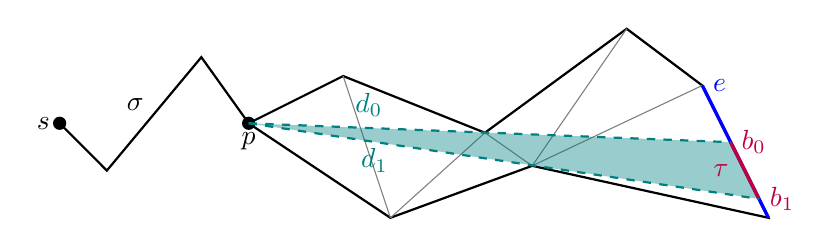
\begin{tikzpicture}[scale=1.2]
			\coordinate (S) at (1,2);
\coordinate (P) at (3,2);
\coordinate (A) at (4,2.5);
\coordinate (B) at (5.5,1.9);
\coordinate (C) at (7,3);
\coordinate (D) at (7.8,2.4);
\coordinate (E) at (8.5,1);
\coordinate (F) at (6,1.55);
\coordinate (G) at (4.5,1);

\coordinate (A0) at (8.1,1.8);
\coordinate (A1) at (8.4,1.2);

% path from source to pseudo-source
\draw[black, thick] (S) -- (1.5, 1.5) -- (2.5, 2.7) -- (P);
\fill (S) circle (0.07) node[left] {$s$};
\fill (P) circle (0.07) node[below] {$p$};
\node at (1.8, 2.2) {$\sigma$};

\draw[black, thick] (P) -- (A) -- (B) -- (C) -- (D) -- (E) -- (F) -- (G) -- (P);
\begin{scope}[gray]
    \draw (A) -- (G);
    \draw (B) -- (G);
    \draw (B) -- (F);
    \draw (C) -- (F);
    \draw (D) -- (F);
\end{scope}

\fill[teal, opacity=0.4] (P) -- (A0) -- (A1) -- cycle;
\draw[blue, very thick] (D) node[right] {$e$} -- (E);
\draw[purple, very thick] (A0) node[right] {$b_0$} -- (A1) node[right] {$b_1$};

\draw[dashed, teal, thick] (P) -- (A0) node[pos=.2, above right] {$d_0$};
\draw[dashed, teal, thick] (P) -- (A1) node[pos=.2, below right] {$d_1$};
\node[purple] at (8, 1.5) {$\tau$};
		\end{tikzpicture}
		\caption{Illustration of a window $w=(s, p, {\color{blue}e}, {\color{purple}b_0}, {\color{purple}b_1}, {\color{teal}d_0}, {\color{teal}d_1}, \sigma)$.}
		\label{fig:ich-windows}
	\end{figure}
\end{frame}

\begin{frame}{One Angle, One Split Rule}
	\begin{figure}[ht]
		\centering
		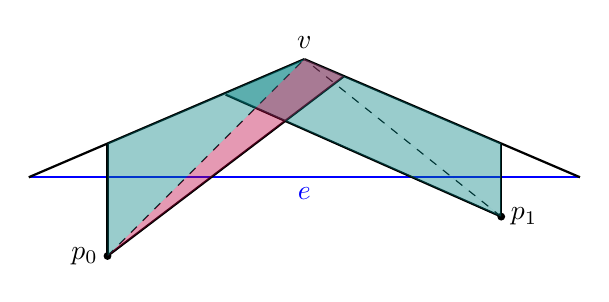
\begin{tikzpicture}
			\coordinate (P0) at (1, -1);
\coordinate (P1) at (6, -0.5);
\coordinate (v) at (3.5, 1.5);
\coordinate (a0) at (1, .43);
\coordinate (a1) at (4, 1.28);
\coordinate (b0) at (2.5, 1.05);
\coordinate (b1) at (6, .43);

\draw[blue, thick] (0, 0) -- (7, 0) node[midway, below] {$e$};
\draw[thick] (0,0) -- (v) node[above] {$v$};
\draw[thick] (7,0) -- (v);

\fill (P0) circle (0.05) node[left] {$p_0$};
\fill (P1) circle (0.05) node[right] {$p_1$};

\draw[thick] (P0) -- (a0);
\draw[thick] (P0) -- (a1);
\draw[thick] (P1) -- (b0);
\draw[thick] (P1) -- (b1);

\draw[dashed] (P0) -- (v);
\draw[dashed] (P1) -- (v);

\fill[teal, opacity=0.4] (P0) -- (a0) -- (v) -- cycle;
\fill[teal, opacity=0.4] (P1) -- (b0) -- (v) -- cycle;
\fill[teal, opacity=0.4] (P1) -- (v) -- (b1) -- cycle;
\fill[purple, opacity=0.4] (P0) -- (v) -- (a1) -- cycle;
		\end{tikzpicture}
		\caption{Illustration of the ``one angle, one split'' pruning rule: only keep three out of four windows.}
		\label{fig:one-angle-one-split}
	\end{figure}
\end{frame}

\begin{frame}{Window Filtering}
	\begin{figure}[ht]
		\centering
		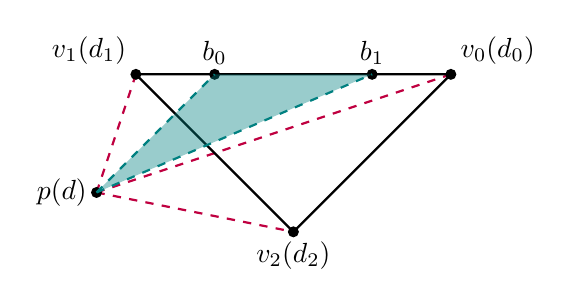
\begin{tikzpicture}
			\coordinate (v0) at (4, 2);
\coordinate (v1) at (0, 2);
\coordinate (v2) at (2, 0);
\coordinate (A) at (3, 2);
\coordinate (B) at (1, 2);
\coordinate (p) at (-0.5, 0.5);

\draw[dashed, thick, purple] (p) -- (v0);
\draw[dashed, thick, purple] (p) -- (v1);
\draw[dashed, thick, purple] (p) -- (v2);

\fill (v0) circle (0.07) node[above right] {$v_0(d_0)$};
\fill (v1) circle (0.07) node[above left] {$v_1(d_1)$};
\fill (v2) circle (0.07) node[below] {$v_2(d_2)$};
\draw[thick] (v0) -- (v1) -- (v2) -- cycle;

\fill (A) circle (0.07) node[above] {$b_1$};
\fill (B) circle (0.07) node[above] {$b_0$};

\fill (p) circle (0.07) node[left] {$p(d)$};
\fill[teal, opacity=0.4] (p) -- (A) -- (B) -- cycle;
\draw[dashed, thick, teal] (p) -- (A);
\draw[dashed, thick, teal] (p) -- (B);
		\end{tikzpicture}
		\label{fig:window-trimming}
	\end{figure}
	We can discard a window $w$ if:
	\begin{itemize}
		\item $d+\norm{pb_0} > d_0 + \norm{v_0b_1}$
		\item $d+\norm{pb_1} > d_1 + \norm{v_1b_1}$
		\item $d+\norm{pb_0} > d_2 + \norm{v_2b_0}$
	\end{itemize}
\end{frame}

\section{Experiments}

\begin{frame}{Compute Time I}
	\begin{figure}
		\includegraphics[width=\textwidth]{../report/images/heat_benchmark.pdf}
		\caption{Benchmark of the \emph{Heat method} as a function of the number of vertices.
		Slope: $2.63$, $r^2$: $0.99$.}
	\end{figure}
\end{frame}

\begin{frame}{Compute Time II}
	\begin{figure}
		\includegraphics[width=\textwidth]{../report/images/fastmarching_benchmark.pdf}
		\caption{Benchmark of the \emph{Fast Marching algorithm} as a function of the number of vertices.
		Slope: $1.51$, $r^2$: $0.98$.}
	\end{figure}
\end{frame}

\begin{frame}{Compute Time III}
	\begin{figure}	
		\includegraphics[width=\textwidth]{../report/images/ich_benchmark.pdf}
		\caption{Benchmark of the \emph{ICH algorithm} as a function of the number of vertices.
		Slope: $1.60$, $r^2$: $0.96$.}
	\end{figure}
\end{frame}

\begin{frame}{Comparison of methods}
	\begin{tblr}[expand=\intertitre]{%
		rowspec={Q[m]Q[m]Q[m]Q[m]Q[m]Q[m]Q[m]Q[m]},
		colspec={Q[co=1,c]Q[co=1.5,mode=math,c, font=\scriptsize]Q[mode=math,co=1.5,c,font=\scriptsize]Q[co=1.2,c]Q[c, co=1.5, font=\scriptsize]},
		hlines = {solid},
		vline{1, 2, 6} = {solid},
		vline{3, 4, 5} = {1}{solid},
		vline{3, 4, 5} = {2-Z}{dashed},
		row{3, 5, 8}={bg=teal!20!white},
				row{1} = {c,font=\bfseries,mode=text,fg=white,bg=teal},
				colsep = 3pt
			}%
		Method        & Theoretical Runtime & Actual Runtime                              & Precision & \small Limitations                                              \\
		\intertitre{PDE-based methods}                                                                                                                                  \\
		Heat          & \O(\nv^{\omega})    & \underset{\nv \to \infty}{\O(\nv^{\omega})} & Approx.   & Stability, runtime, fixed sources, no paths                     \\
		Poisson       & \O(\nv^{\omega})    &                                             & Approx.   & Stability, not true geodesics, runtime, fixed sources, no paths \\
		Spectral      & \O(\nv^{\omega})    &                                             & Approx.   & Stability, not true geodesics, runtime, no paths                \\
		Fast Marching & \O(\nv\log \nv)     & \O(\nv^{1.5})                               & Approx.   & Fixed sources, limited to meshes, no paths                      \\
		\intertitre{Computational geometry methods}                                                                                                                     \\
		ICH           & \O(\nv^{2}\log \nv) & \O(\nv^{1.6})                               & Exact     & Limited to meshes, fixed (but possibly non-edge) sources
	\end{tblr}
\end{frame}

\appendix
\begin{frame}[allowframebreaks]
	\frametitle{Bibliography}
	\printbibliography
\end{frame}
\end{document}
